% Sablon pentru realizarea lucrarii de licenta, conform cu recomandarile
% din ghidul de redactare:
% - https://fmi.unibuc.ro/finalizare-studii/

% Multumiri lui Gabriel Majeri, acest sablon a fost creat pe baza
% codului sursa a lucrarii sale de licenta. 
% Codul sursa: https://github.com/GabrielMajeri/bachelors-thesis
% Website: https://www.gabrielmajeri.ro/
%
% Acest sablon este licentiat sub Creative Commons Attribution 4.0 International License.
% modificat 8 noiembrie 2024

\documentclass[12pt, a4paper]{article}

% Suport pentru diacritice și alte simboluri
\usepackage{fontspec}

% Font Times New Roman
\usepackage{times}

% Suport pentru mai multe limbi
\usepackage{polyglossia}

% Setează limba textului la română
\setdefaultlanguage{romanian}
% Am nevoie de engleză pentru rezumat
\setotherlanguages{english}

% Indentează și primul paragraf al fiecărei noi secțiuni
\SetLanguageKeys{romanian}{indentfirst=true}

% Suport pentru diferite stiluri de ghilimele
\usepackage{csquotes}

\DeclareQuoteStyle{romanian}
  {\quotedblbase}
  {\textquotedblright}
  {\guillemotleft}
  {\guillemotright}

% Utilizează biblatex pentru referințe bibliografice
\usepackage[
    maxbibnames=50,
    sorting=nty
]{biblatex}

\addbibresource{bibliography.bib}

% Setează spațiere inter-linie (doublespacing din LaTeX este echivalentul setarii 1.5 in Microsoft Word)
\usepackage{setspace}
\doublespacing

% Modificarea geometriei paginii (cu margini de 2,5 cm) 
\usepackage[margin=2.5cm]{geometry}

% Include funcțiile de grafică
\usepackage{graphicx}
% Încarcă imaginile din directorul `images`
\graphicspath{{./images/}}

% Listări de cod
\usepackage{listings}

% Pseudocod cu formatare matematică
\usepackage[ruled, vlined, linesnumbered]{algorithm2e}
\SetKwInput{KwData}{Date de intrare}
\SetKwInput{KwResult}{Rezultat}
\SetKwFor{For}{pentru}{execută}{sfârșit}
\SetKwFor{ForEach}{pentru fiecare}{execută}{sfârșit}
\SetKwRepeat{Repeat}{repetă de}{ori}
\SetKwFunction{FPermutare}{permutare}
\SetKwProg{Fn}{Funcția}{:}{}
% cuvinte-cheie traduse în română
\SetKw{KwTo}{până la}
\SetKwIF{If}{ElseIf}{Else}{dacă}{atunci}{altfel dacă}{altfel}{sfârșit}
\SetKwFor{While}{cât timp}{execută}{sfârșit}
\renewcommand{\algorithmcfname}{Algoritmul}
% rotație circulară spre stânga
\newcommand{\rotl}[2]{#1 \lll #2}

% Linkuri interactive în PDF
\usepackage[
    colorlinks,
    linkcolor={black},
    menucolor={black},
    citecolor={black},
    urlcolor={blue}
]{hyperref}

% Simboluri matematice codificate Unicode
\usepackage[warnings-off={mathtools-colon,mathtools-overbracket}]{unicode-math}

% Comenzi matematice
\usepackage{amsmath}
\usepackage{mathtools}

% Formule matematice
\newcommand{\bigO}[1]{\symcal{O}\left(#1\right)}
\DeclarePairedDelimiter\abs{\lvert}{\rvert}

% Suport pentru rezumat în două limbi
% Bazat pe https://tex.stackexchange.com/a/70818
\newenvironment{abstractpage}
  {\cleardoublepage\vspace*{\fill}\thispagestyle{empty}}
  {\vfill\cleardoublepage}
\renewenvironment{abstract}[1]
  {\bigskip\selectlanguage{#1}%
   \begin{center}\bfseries\abstractname\end{center}}
  {\par\bigskip}

% Suport pentru anexe
\usepackage{appendix}

% Stiluri diferite de headere și footere
\usepackage{fancyhdr}

% Metadate
\title{O funcție hash paralelizabilă bazată pe sisteme dinamice discrete haotice}
\author{Aelenei Alex-Ioan}

% Generează variabilele cu @
\makeatletter

\begin{document}

% Front matter
\cleardoublepage
\let\ps@plain

% Pagina de titlu
\include{0-title}
\restoregeometry
\newgeometry{
    margin=2.5cm
}

\fancypagestyle{main}{
  \fancyhf{}
  \renewcommand\headrulewidth{0pt}
  \fancyhead[C]{}
  \fancyfoot[C]{\thepage}
}

\addtocounter{page}{1}

% Rezumatul
\begin{abstractpage}

\begin{abstract}{romanian}
Abstract aici
\end{abstract}

\begin{abstract}{english}
Rezumat aici
\end{abstract}

\end{abstractpage}

\tableofcontents

% Main matter
\cleardoublepage
\pagestyle{main}
\let\ps@plain\ps@main

\section{Introducere}

În societatea contemporană, influența dezvoltărilor mijloacelor de calcul este incontestabilă și se resfrânge asupra tuturor aspectelor vieții.
Acest impact semnificativ nu este unul întâmplător, ci rezultatul a decenii de inovații.
Două arii conexe care s-au remarcat timpuriu a fi semnificative în această evoluție au fost criptografia și criptanaliza. \\

Asemănător cu orice alt domeniu, pe parcursul timpului, în criptografie, au apărut o serie de provocări și puncte vulnerabile, dintre acestea evidențiindu-se: autentificarea și integritatea datelor.
Autentificarea asigură veridicitatea identității iar integritatea datelor garantează absența modificărilor nedorite.
În acest context, se remarcă funcțiile hash, un instrument criptografic cu aplicații variate.
Însăși definiția funcției hash demonstrează caracterul versatil al utilității sale: transformă un șir de lungime arbitrară într-un șir de lungime fixă.
Unidirecționalitatea funcției hash determină practicalitatea acesteia.
Începând sfărșitul celui de-al doilea mileniu, numeroase structuri de funcții hash au fost propuse și analizate.
Prima generație de funcții hash moderne a fost reprezentată de MD5~\cite{rivest1992md5}, bazată pe construcția Merkle-Damgård~\cite{merkle1989,damgard1989}.
Vulnerabilitățile acestei funcții la atacurile cu preimagine sau extinderea lungimii mesajului au devenit rapid evidente.
În consecință, au urmat două alte iterații menite să adreseze problemele MD5: SHA-1~\cite{nist1995sha1} și SHA-2~\cite{nist2015sha2}.
SHA-1 a fost ulterior compromisă, dar SHA-2 rămâne în continuare standardul la nivel de industrie.
În ciuda adoptării generalizate, SHA-2 este fundamentată pe aceeași construcție Merkele-Damgård.
Defectele structurale ale acestei construcții au fost relevate de timp.
Construcția s-a dovedit vulnerabilă la o multitidudine de atacuri, inclusiv cele cu preimagine și extinderea lungimii mesajului.
Având în vedere acest context, apariția SHA-3 a fost inevitabilă.
Structura SHA-3 se îndepărtează de structura definită de Merkle și Damgård, și adoptă construcția sponge~\cite{bertoni2007sponge}. \\

În procesul de confuzie și difuzie caracteristic funcțiilor hash~\cite{shannon1949}, se remarcă numeroase de structuri și construcții.
Majoritatea funcțiilor hash moderne se bazează pe substituții, transpoziții, permutări și operații aritmetice.
Aceste metode sunt eficiente, însă proprietățile lor criptografice nu sunt garantate de un model matematic unitar.
Mularea pe o serie de criterii statistice, fără a exista o garanție structurală produce un efect de avalanșă incert, întrucât implică o serie de ipoteze și presupuneri care, în eventualitatea unei vulnerabilități, pot fi invalidate sau propagate la dependenți.
Un instrument care conferă prin definiție confuzie și difuzie este reprezentat de sistemele dinamice haotice~\cite{alvarez2006}, o subcategorie a sistemelor dinamice discrete.
Un astfel de sistem descrie o transformare deterministă care pare complet predictibilă la o primă inspecție, însă, în realitate, manifestă un comportament complex și aparent aleator, caracterizat de o sensibilitate extremă la condițiile inițiale.
Aceste sisteme prezintă trei proprietăți definitorii care se aliniază remarcabil cu cerințele criptografice formulate de Shannon~\cite{shannon1949,devaney1989,alvarez2006}.
Prima este tranzitivitatea topolgică, iar a doua este densitatea orbitelor periodice.
Cea de a treia proprietate, sensibilitatea la condițiile inițiale, este asigurată de primele două proprietăți~\cite{banks1992}.
Astfel, faptul că securitatea sistemelor haotice nu se întemeiază pe nicio construcție euristică este esențial.
Absența unei structuri algebrice exploatabile, asociată de regulă cu vulnerabilitatea la atacurile cuantice, transformă această aparentă lipsă de structură într-un atu de securitate.

Având în vedere aceste considerente, lucrarea de față propune o nouă funcție hash bazată pe sisteme dinamice discrete haotice.
Securitatea acestei funcții hash se bazează pe proprietățile sistemelor haotice îmbinate cu tehnicile clasice de confuzie și difuzie.
Ce diferențiază această funcție hash de cele existente este structura optimizată pentru procesare paralelă.
Folosindu-se de arbori Merkle și de construcția sponge, această funcție hash are o performanță superioară în comparație cu alte funcții similare.
Valorificând sistemele hardware moderne multicore, această funcție are o viteză de procesare care o face utilizabilă în scenarii de producție. \\

În continuare, în Capitolul 2 vor fi prezentate sistemele haotice utilizate în această lucrare.
Capitolul 3 va include o descriere exhaustivă a arhitecturii funcției hash propuse, împreună cu o implementare în pseudocod a funcției.
În capitolul 4 va fi prezentată atât analiza criptografica a funcției hash, cât și analiza performanței acesteia, mai ales în comparație cu alte funcții hash similare.
În final, în capitolul 5 vor fi prezentate concluziile și viitoare direcții de dezvoltare.
\section{Preliminarii}

\subsection{Funcția hash}

O funcție hash criptografică este o transformare deterministă $h \colon \{0,1\}^* \to \{0,1\}^n$ care asociază datelor de intrare de lungime arbitrară un hash de lungime fixă $n$.
Pentru a fi utilă în context criptografic, ea trebuie să fie eficientă din punct de veder computațional și să satisfacă trei proprietăți de securitate ~\cite{merkle1989, damgard1989}: 
\begin{enumerate}
    \item Rezistența la preimagine: dat fiind un hash $y$, este infezabil să se găsească un mesaj $m$ cu $h(m) = y$.
    \item Rezistența la a doua preimagine: dat un mesaj $m$, este infezabil să se găsească $m' \neq m$ cu $h(m') = h(m)$.
    \item Rezistența la coliziuni: este infezabil să se găsească orice pereche $m \neq m'$ cu $h(m) = h(m')$.
\end{enumerate}

\subsection{Sistemul dinamice}

Un sistem dinamic discret este un triplet $(T, X, f)$, unde:
\begin{enumerate}
    \item $T$ este spațiul timpului, iar $(T, +)$ este un monoid aditiv
    \item $X$ este spațiul de stări sau spațiul fazelor
    \item $f \colon T \times X \to X$ este funcția de evoluție, care satisface următoarele condiții:
    \begin{enumerate}
        \item $f(0, x) = x$
        \item $f(t+s, x) = f(t, f(s, x))$ pentru orice $t, s \in T$ și $x \in X$
    \end{enumerate}
\end{enumerate}
Devaney ~\cite{devaney1989} definește un sistem haotic ca având trei proprietăți esențiale: sensibilitate la condițiile inițiale, tranzitivitate topologică și faptul că mulțimea orbitelor periodice este densă. 
Banks ~\cite{banks1992} demonstrează că tranzitivitatea topologică și densitatea orbitelor periodice implică sensibilitatea la condițiile inițiale. \\

Exponentul Lyapunov măsoară rata medie de separare exponențială a două orbite pornite din condiții inițiale infinitezimal de apropiate.
Pentru un sistem unidimensional cu funcția de evoluție $f$, el este definit ca:
\begin{equation}
    \lambda = \lim_{N \to \infty} \frac{1}{N} \sum_{k=0}^{N-1} \ln \abs{f'(x_k)},
\end{equation}
unde $x_k$ sunt iteratele orbitei.
O valoare $\lambda > 0$ indică divergența exponențială a orbitelor vecine și constituie semnătura cantitativă a comportamentului haotic, în timp ce $\lambda \le 0$ corespunde unei dinamici stabile sau cvasi-periodice~\cite{devaney1989, alvarez2006}. \\

Relevanța exponentului Lyapunov pentru o funcție hash reiese tocmai din această sensibilitate la condițiile inițiale.
Un exponent strict pozitiv garantează că modificarea unui singur bit din datele de intrare se propagă exponențial pe parcursul iterațiilor, separând rapid orbitele corespunzătoare a două mesaje aproape identice.
Acest mecanism stă la baza efectului de avalanșă dorit, prin care date de intrare cu diferențe minime produc hash-uri complet necorelate, iar magnitudinea exponentului oferă o măsură cantitativă a vitezei cu care difuzia atinge saturația~\cite{alvarez2006}. \\

\subsection{Construcția Sponge}

Construcția Sponge este o schemă de proiectare a funcțiilor hash care operează asupra unei stări interne de lățime $b$ biți.
Starea internă este împărțită într-o rată $r$ și o capacitate $c$.
Asupra stării interne se aplică în mod repetat o permutare fixă $f$~\cite{bertoni2007sponge}.
Procesarea se desfășoară în două faze: în faza de absorbție, blocurile mesajului, de câte $r$ biți, sunt XOR-ate cu partea de rată a stării.
Ulterior se aplică permutarea $f$. 
În faza de stoarcere, biții pentru hash sunt extrași din partea de rată, intercalați cu aplicări succesive ale lui $f$, până la obținerea lungimii dorite a hash-ului.
Capacitatea $c$, care nu este expusă niciodată direct la intrare sau la ieșire, determină nivelul de securitate al construcției. \\

\begin{figure}[ht]
    \centering
    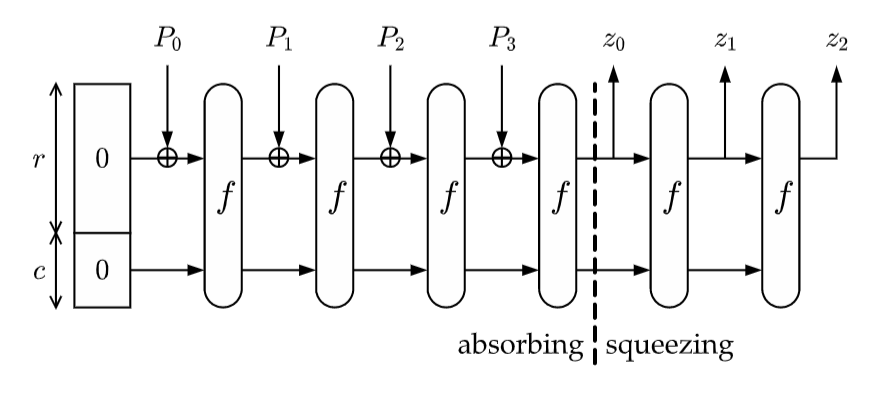
\includegraphics[width=0.8\textwidth]{sponge.png}
    \caption{Construcția Sponge ~\cite{bertoni2007sponge}.}
    \label{fig:sponge}
\end{figure}

\subsection{Arborele Merkle}

Arborele Merkle este o structură de date arborescentă, de regulă binară, în care fiecare frunză conține hash-ul unui bloc de date.
Fiecare nod intern conține hash-ul obținut prin concatenarea și aplicarea funcției hash asupra hash-urilor copiilor săi~\cite{merkle1989}.
Hash-ul nodului rădăcină, numit rădăcină Merkle, sintetizează astfel întregul set de date într-o singură valoare de lungime fixă.
Orice modificare a unui bloc se propagă în mod inevitabil până la rădăcină.
Această organizare permite paralelizarea funcțiilor hash, întrucât subarborii independenți pot fi procesați simultan. \\

\section{Funcția haotică}

Nucleul funcției hash propuse îl constituie o transformare haotică aplicată repetat asupra stării interne.
Această transformare nu se reduce la o singură funcție, ci la suprapunerea a două sisteme dinamice distincte, alese astfel încât slăbiciunile fiecăruia să fie compensate de celălalt.
Prima este baker's map, responsabilă de difuzie, iar a doua este gingerbreadman map, responsabilă de confuzie.
Compunerea lor produce, la fiecare iterație, atât amestecarea uniformă a stării, cât și o neliniaritate suficientă pentru a împiedica orice descriere algebrică simplă a procesului. \\

\subsection{Exponentul Lyapunov}

Afirmația că o funcție manifestă un comportament haotic poate fi cuantificată riguros prin intermediul exponentului Lyapunov.
Acesta măsoară rata medie cu care două traiectorii pornite din condiții inițiale infinit de apropiate se îndepărtează una de cealaltă.
Fie două puncte de start separate de o perturbație inițială $\delta_0$.
Pentru un sistem haotic, distanța dintre traiectoriile lor crește, în medie, exponențial cu numărul de iterații $n$:

\begin{equation}
    \abs{\delta_n} \approx \abs{\delta_0} \, e^{\lambda n}
\end{equation}

Coeficientul $\lambda$ din exponent este tocmai exponentul Lyapunov.
O valoare pozitivă, $\lambda > 0$, indică divergența exponențială a traiectoriilor și, implicit, sensibilitatea extremă la condițiile inițiale specifică haosului.
O valoare negativă indică, dimpotrivă, convergența traiectoriilor către o orbită stabilă. \\

\subsubsection{Liniarizarea prin matricea jacobiană}

Pentru a măsura această divergență, perturbația $\delta$ nu se urmărește prin reaplicarea funcției asupra a două puncte distincte, deoarece, după câțiva pași, distanța dintre ele depășește domeniul în care aproximarea liniară este validă.
În schimb, evoluția unei perturbații infinitezimale este descrisă de liniarizarea funcției în jurul punctului curent al traiectoriei.
Fie funcția bidimensională $F(x, y) = \left( f(x, y),\ g(x, y) \right)$.
Liniarizarea sa în punctul $p_n = (x_n, y_n)$ este dată de matricea jacobiană, care conține derivatele parțiale ale componentelor funcției:

\begin{equation}
    J(p_n) =
    \begin{pmatrix}
        \frac{\partial f}{\partial x} & \frac{\partial f}{\partial y} \\[6pt]
        \frac{\partial g}{\partial x} & \frac{\partial g}{\partial y}
    \end{pmatrix}_{p_n}
\end{equation}

Aplicată unui vector tangent $v$ (o perturbație infinitezimală), matricea jacobiană indică modul în care acel vector este rotit și scalat de o singură iterație a funcției.
Astfel, evoluția perturbației de-a lungul orbitei se reduce la o înmulțire matrice-vector la fiecare pas:

\begin{equation}
    v_{n+1} = J(p_n) \, v_n
\end{equation}

După $N$ iterații, vectorul tangent inițial $v_0$ este transformat prin produsul matricelor jacobiene evaluate succesiv în lungul traiectoriei:

\begin{equation}
    v_N = J(p_{N-1}) \, J(p_{N-2}) \cdots J(p_0) \, v_0
\end{equation}

Exponentul Lyapunov se obține ca rata medie de creștere logaritmică a normei vectorului tangent, pe măsură ce numărul de pași tinde la infinit:

\begin{equation}
    \lambda = \lim_{N \to \infty} \frac{1}{N} \ln \frac{\abs{v_N}}{\abs{v_0}}
\end{equation}

\subsubsection{Spectrul Lyapunov al unui sistem bidimensional}

Un sistem bidimensional nu posedă un singur exponent, ci un spectru de doi exponenți, $\lambda_1 \geq \lambda_2$, câte unul pentru fiecare direcție independentă a spațiului de stări.
Aceștia descriu deformarea unui disc infinitezimal de condiții inițiale: $\lambda_1$ caracterizează direcția de întindere maximă, iar $\lambda_2$ direcția de contracție.
Cel mai mare exponent, $\lambda_1$, domină comportamentul pe termen lung, fiindcă orice vector tangent ales aleatoriu se aliniază rapid direcției de creștere maximă; pozitivitatea sa este criteriul standard pentru identificarea haosului.
Suma celor doi exponenți este legată de variația ariei sub acțiunea funcției, prin logaritmul determinantului jacobian:

\begin{equation}
    \lambda_1 + \lambda_2 = \lim_{N \to \infty} \frac{1}{N} \sum_{n=0}^{N-1} \ln \abs{\det J(p_n)}
\end{equation}

Pentru o funcție care conservă aria, precum gingerbreadman map, această sumă este nulă: orice întindere pe o direcție este compensată exact de o contracție pe cealaltă.

\subsubsection{Estimarea numerică}

Calculul direct al produsului de matrice jacobiene este instabil numeric.
Deoarece toți vectorii tangenți tind să se alinieze direcției dominante, al doilea exponent devine imposibil de recuperat, iar normele cresc sau scad necontrolat, conducând la depășiri de domeniu.
Soluția standard este algoritmul lui Benettin~\cite{benettin1980}, care propagă simultan doi vectori tangenți ortonormali și îi re-ortonormalizează periodic prin procedeul Gram-Schmidt.
La fiecare pas, înainte de re-ortonormalizare, se acumulează logaritmul factorilor de creștere ai celor doi vectori; mediile acestor logaritmi, raportate la numărul de pași, converg către cei doi exponenți Lyapunov.

\begin{algorithm}[H]
    \KwData{Funcția $F$, jacobianul $J$, punctul inițial $p_0$, numărul de pași $N$}
    \KwResult{Exponenții Lyapunov $\lambda_1, \lambda_2$}
    inițializează $v_1 \gets (1, 0)$, $v_2 \gets (0, 1)$\;
    inițializează $s_1 \gets 0$, $s_2 \gets 0$\;
    \For{$n \gets 0$ \KwTo $N - 1$}{
        $v_1 \gets J(p_n) \, v_1$\;
        $v_2 \gets J(p_n) \, v_2$\;
        $r_1 \gets \abs{v_1}$;\quad $v_1 \gets v_1 / r_1$\;
        $v_2 \gets v_2 - (v_2 \cdot v_1) \, v_1$\;
        $r_2 \gets \abs{v_2}$;\quad $v_2 \gets v_2 / r_2$\;
        $s_1 \gets s_1 + \ln r_1$;\quad $s_2 \gets s_2 + \ln r_2$\;
        $p_{n+1} \gets F(p_n)$\;
    }
    $\lambda_1 \gets s_1 / N$;\quad $\lambda_2 \gets s_2 / N$\;
    \caption{Estimarea spectrului Lyapunov~\cite{benettin1980}}
\end{algorithm}

\subsection{Baker's map}

Baker's map este un sistem dinamic clasic~\cite{devaney1989}, a cărui denumire provine dintr-o analogie sugestivă cu procesul de frământare a aluatului.
Brutarul întinde aluatul pe o direcție, dublându-i lungimea, după care îl pliază la loc peste sine.
Repetarea acestui gest amestecă rapid și ireversibil orice particulă din interiorul aluatului, dispersând-o în întreaga masă.
Formal, sistemul dinamic are următoarea relație de recurență:

\begin{equation}
    (x_{n+1}, y_{n+1}) =
    \begin{cases}
        (2x_n, \frac{y_n}{2}) & \text{dacă } 0 \leq x_n < \frac{1}{2} \\
        (2 - 2x_n, 1 - \frac{y_n}{2}) & \text{dacă } \frac{1}{2} \leq x_n < 1
    \end{cases}
\end{equation}

\subsection{Gingerbreadman map}

Gingerbreadman map, introdusă de Devaney~\cite{devaney1989}, este un sistem dinamic haotic bidimensional.
Numele său provine din forma caracteristică a atractorului, care, vizualizat în plan, amintește de silueta unei figurine din turtă dulce.
Definitorie pentru această funcție este prezența valorii absolute, singura sursă de neliniaritate. \\
Formal, sistemul dinamic are următoarea relație de recurență:

\begin{equation}
    (x_{n+1}, y_{n+1}) = (1-y_n + \abs{x_n}, x_n)
\end{equation}

\subsection{Suprapunerea celor două funcții}

Cele două sisteme se completează reciproc tocmai prin slăbiciunile lor complementare.
Baker's map oferă o amestecare uniformă și lipsită de insule de stabilitate, dar este liniară.
Gingerbreadman map oferă neliniaritatea absentă din prima, dar conține regiuni cvasi-periodice.
Aplicată prima, baker's map dispersează punctul pe întregul spațiu de stări.
Astfel, dacă punctul curent se află într-o regiune cvasi-periodică a gingerbreadman map, punctul va fi împins într-o nouă orbită.
Aplicată în continuare, gingerbreadman map împletește neliniar coordonatele astfel decorelate.
În consecință, această rundă compusă, deși complet deterministă, manifestă un comportament haotic, cu o sensibilitate extremă la condițiile inițiale.
Alegerea celor două sisteme a fost motivată de faptul că ambele prezintă un comportament haotic și sunt eficiente din punct de vedere computațional.
Definițiile acestora presupun o implementare cu operații aritmetice simple, fiind utilizate tipuri de date native.

\subsection{Spectrul Lyapunov al funcțiilor}

Pentru a confirma empiric comportamentul haotic descris, spectrul Lyapunov a fost estimat numeric pentru fiecare dintre cele trei funcții, folosind algoritmul lui Benettin aplicat pe un număr mare de condiții inițiale alese aleatoriu.
Figurile următoare reprezintă cei doi exponenți, $\lambda_1$ și $\lambda_2$, codificați cromatic în funcție de valoarea lor, în planul condițiilor inițiale $(x, y)$.

\begin{figure}[!htbp]
    \centering
    \begin{minipage}{0.49\textwidth}
        \centering
        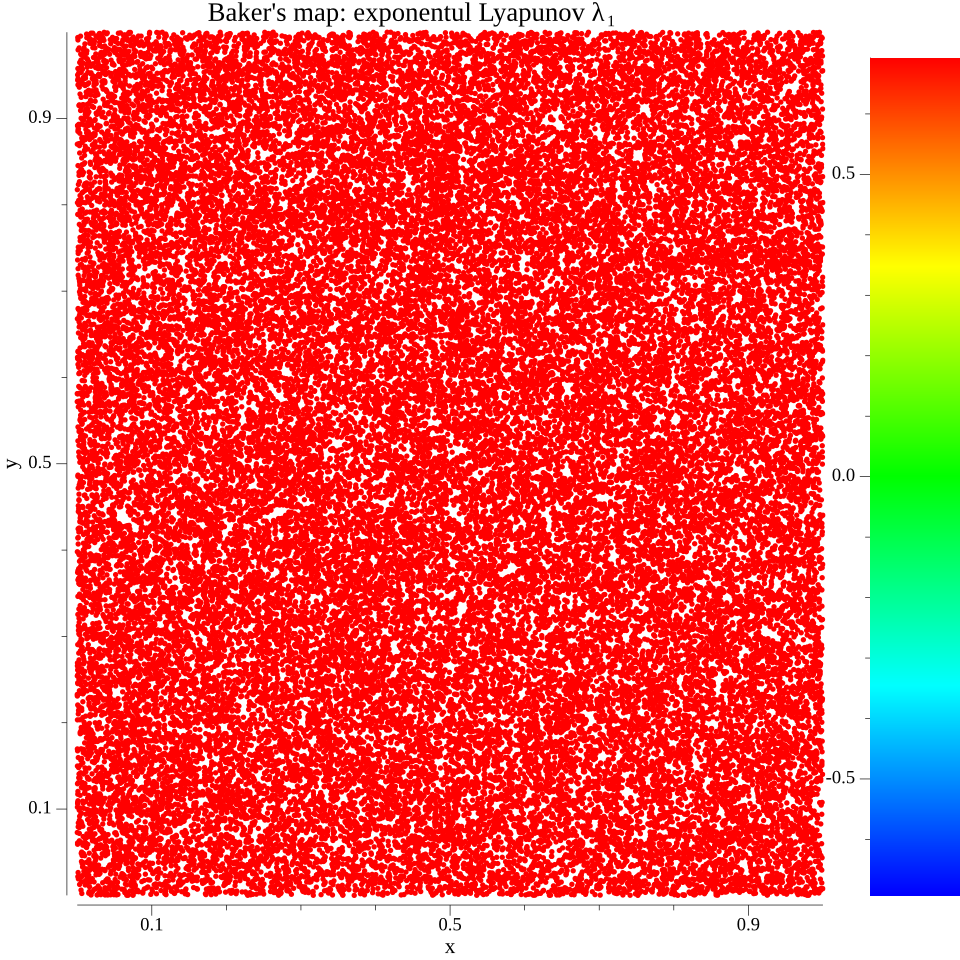
\includegraphics[width=\linewidth]{images/test-chaotic-maps-baker-lambda1.png}
    \end{minipage}
    \hfill
    \begin{minipage}{0.49\textwidth}
        \centering
        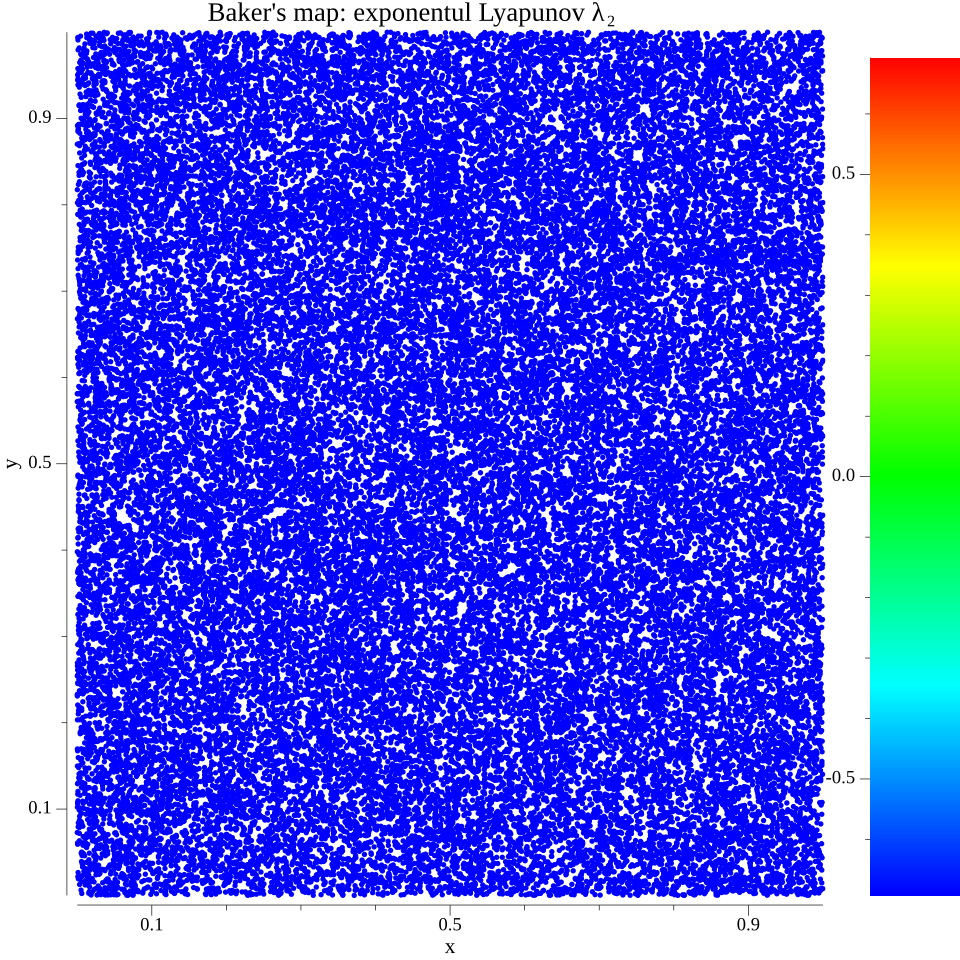
\includegraphics[width=\linewidth]{images/test-chaotic-maps-baker-lambda2.png}
    \end{minipage}
    \caption{Exponenții Lyapunov $\lambda_1$ (stânga) și $\lambda_2$ (dreapta) ai baker's map}
    \label{fig:lyapunov-baker}
\end{figure}

\begin{figure}[!htbp]
    \centering
    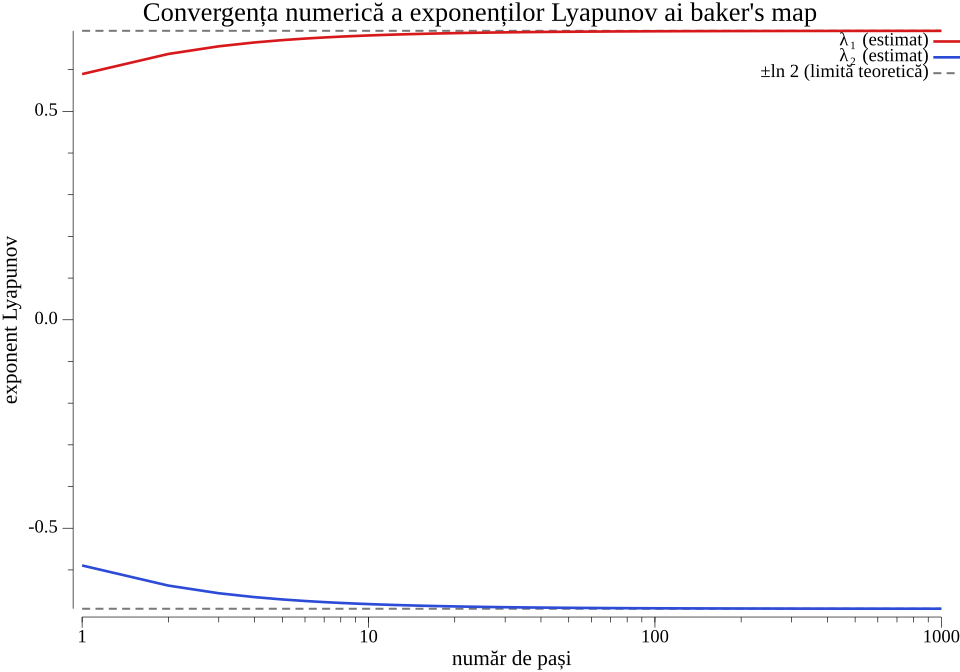
\includegraphics[width=\linewidth]{images/test-chaotic-maps-baker-convergence.png}
    \caption{Convergența numerică a exponenților Lyapunov ai baker's map către limitele teoretice $\pm\ln 2$}
    \label{fig:lyapunov-baker-convergence}
\end{figure}

\begin{figure}[!htbp]
    \centering
    \begin{minipage}{0.49\textwidth}
        \centering
        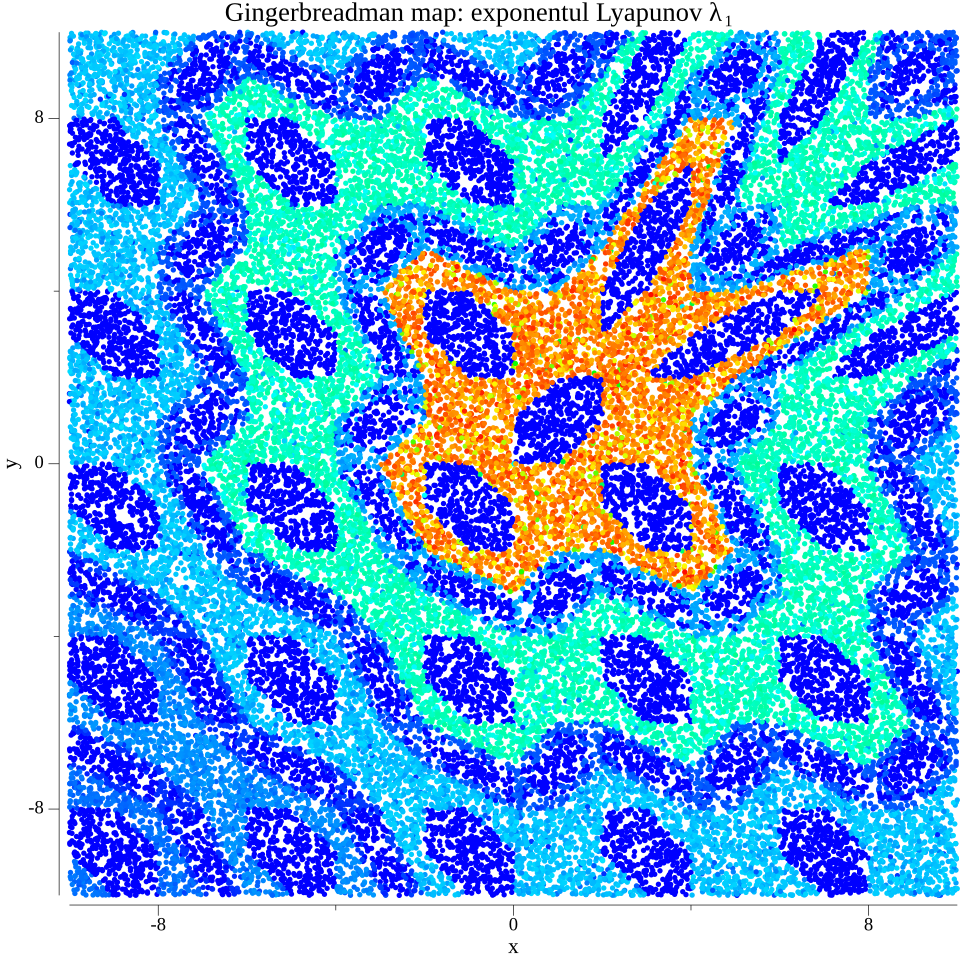
\includegraphics[width=\linewidth]{images/test-chaotic-maps-gingerbreadman-lambda1.png}
    \end{minipage}
    \hfill
    \begin{minipage}{0.49\textwidth}
        \centering
        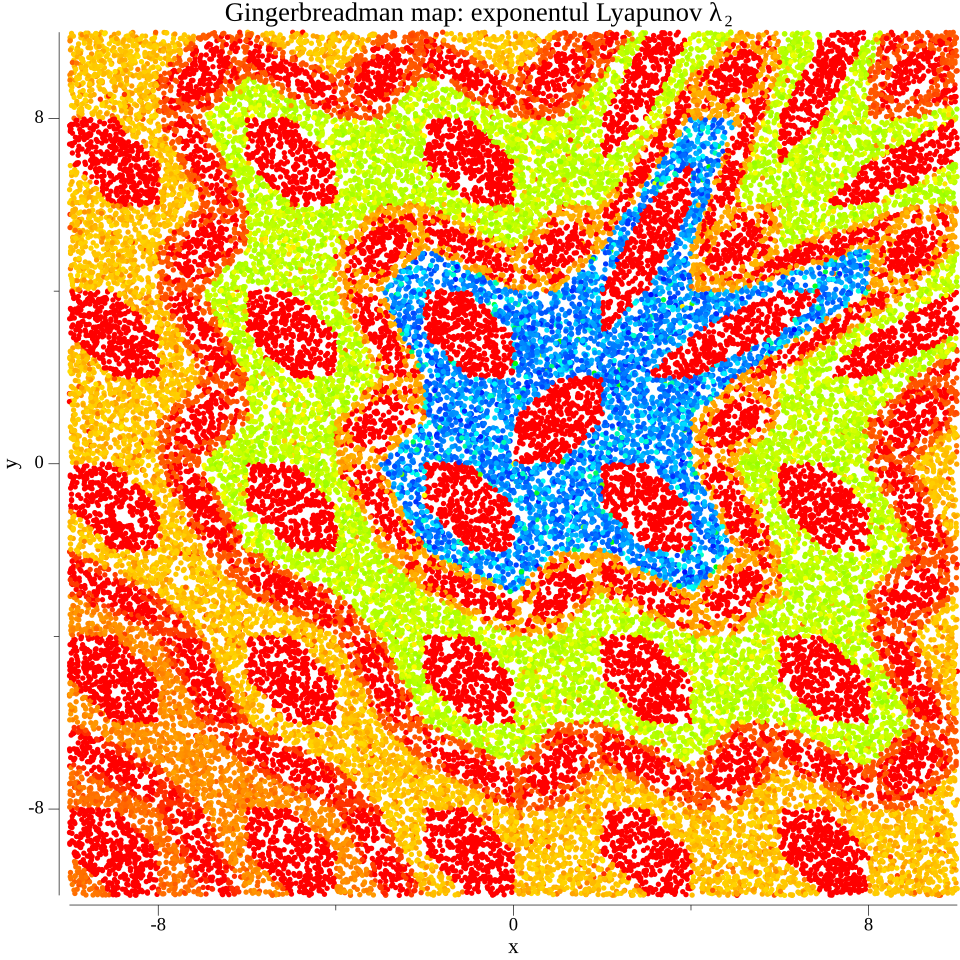
\includegraphics[width=\linewidth]{images/test-chaotic-maps-gingerbreadman-lambda2.png}
    \end{minipage}
    \caption{Exponenții Lyapunov $\lambda_1$ (stânga) și $\lambda_2$ (dreapta) ai gingerbreadman map}
    \label{fig:lyapunov-gingerbreadman}
\end{figure}

\begin{figure}[!htbp]
    \centering
    \begin{minipage}{0.49\textwidth}
        \centering
        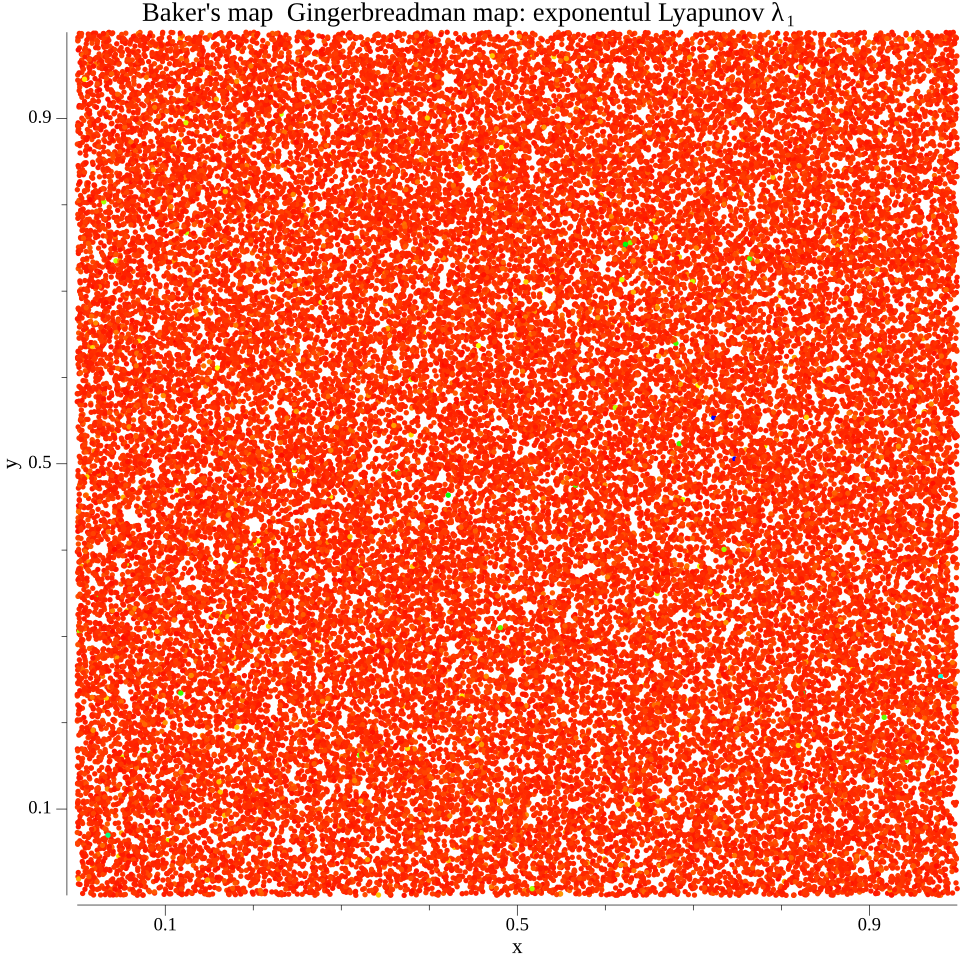
\includegraphics[width=\linewidth]{images/test-chaotic-maps-hash-lambda1.png}
    \end{minipage}
    \hfill
    \begin{minipage}{0.49\textwidth}
        \centering
        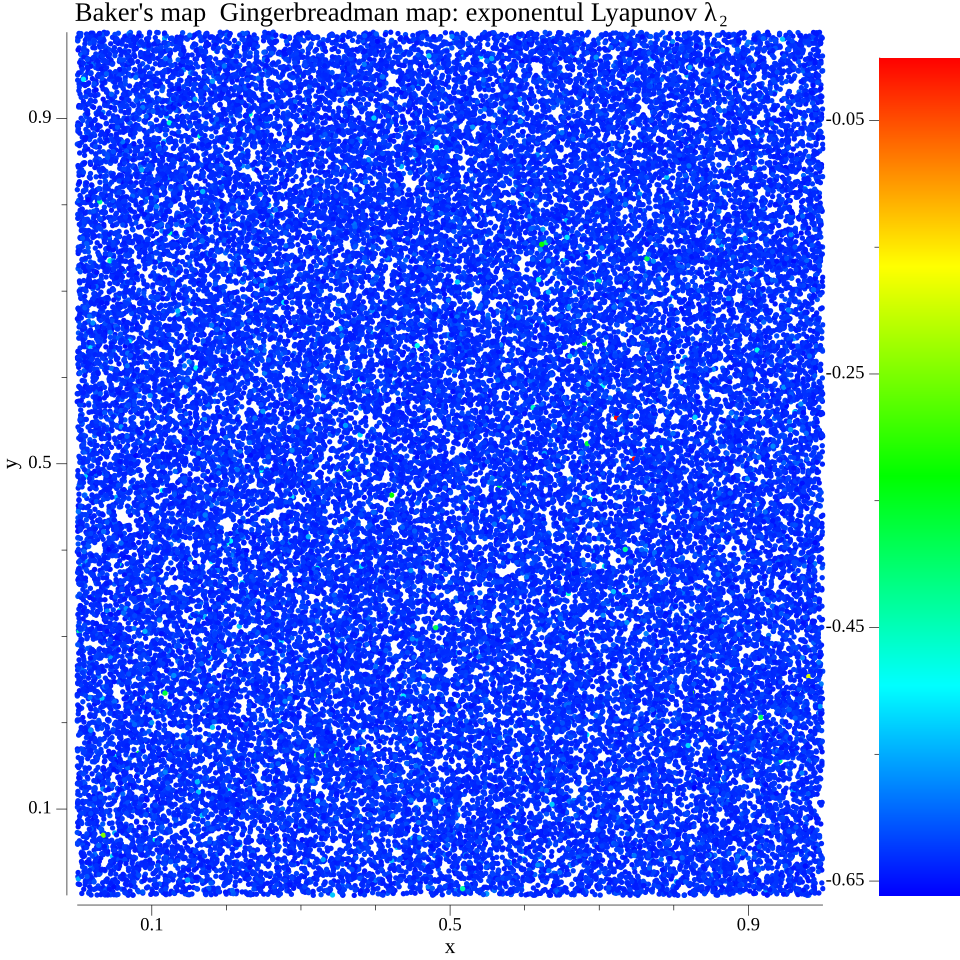
\includegraphics[width=\linewidth]{images/test-chaotic-maps-hash-lambda2.png}
    \end{minipage}
    \caption{Exponenții Lyapunov $\lambda_1$ (stânga) și $\lambda_2$ (dreapta) ai rundei compuse}
    \label{fig:lyapunov-hash}
\end{figure}

\begin{figure}[!htbp]
    \centering
    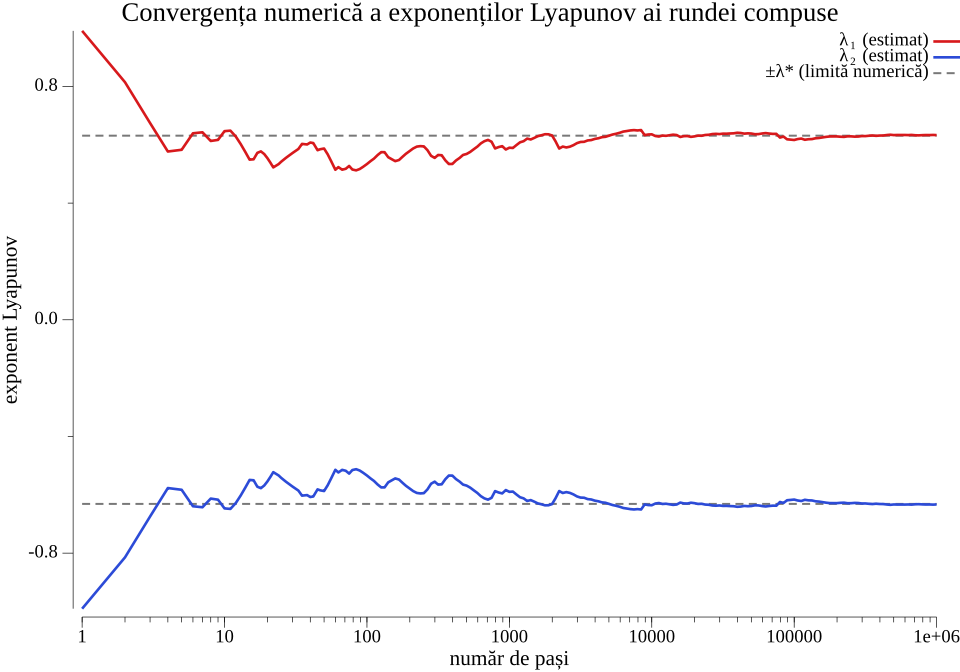
\includegraphics[width=\linewidth]{images/test-chaotic-maps-hash-convergence.png}
    \caption{Convergența numerică a exponenților Lyapunov ai rundei compuse către limita numerică $\pm\lambda^* \approx \pm0{,}6331$}
    \label{fig:lyapunov-hash-convergence}
\end{figure}


\section{Funcția hash}

Funcția hash propusă în această lucrare se bazează pe toate conceptele prezentate în secțiunile anterioare.
Structura Sponge este aplicată pe blocuri, iar apoi prin intermediul arborelui Merkle se obține hash-ul întregului mesaj.
Dimensiunea stării interne este de 1024 biți, împărțită în 512 biți pentru rată și 512 biți de capacitate.
Transformarea internă a stării este realizată printr-o secțiune haotică, completată de metode clasice de confuzie și difuzie. 
Pentru fragmentele următoare de pseudocod, considerăm următoarele convenții de notație:
\begin{itemize}
    \item $S$ reprezintă starea internă, formată din 32 de cuvinte de 32 de biți, $S_i$ fiind cuvântul de pe poziția $i$.
    \item $a \oplus b$ reprezintă XOR-are (disjuncție exclusivă) bit cu bit.
    \item $\rotl{a}{k}$ reprezintă rotația circulară spre stânga a cuvântului $a$ cu $k$ poziții.
    \item $a \bmod b$ reprezintă restul împărțirii lui $a$ la $b$.
    \item $l$ reprezintă lungimea hash-ului final, exprimată în biți.
\end{itemize}

\subsection{Preprocesarea}
Secțiunea de preprocesare are rolul de a pregăti mesajul inițial pentru absorbția în construcția Sponge.
Astfel, lungimea mesajului preprocesat trebuie să fie un multiplu al ratei de 512 biți.
Considerând că mesajul inițial este $M$, alcătuit din $M=M_1 \| M_2 \| \ldots \| M_n$, unde $M_i$ reprezintă un byte, mesajul preprocesat va fi:

\begin{equation}
    M' = M \| \texttt{0x80} \| \texttt{0x00} \| \ldots \| \texttt{0x00} \| \texttt{0x01},
\end{equation}

\subsection{Generarea frunzelor}
După preprocesare, mesajul este împărțit în blocuri de dimensiune configurabilă.
Fiecare bloc $B_i$ va reprezenta o frunză în arborele Merkle, iar hash-ul său va fi calculat prin aplicarea construcției Sponge.
Trebuie menționat faptul că dimensiunea unui bloc este un parametru configurabil.

\subsection{Construcția Sponge}
Construcția Sponge este aplicată pe fiecare bloc $B_i$ pentru a genera hash-ul.
Fiecare bloc de 512 biți este XOR-at cu partea de rată a stării interne, după care se aplică permutarea haotică.
Permutarea $f$ a construcției Sponge este aplicată după fiecare absorbție a unui bloc.
Starea internă este împărțită în 16 secțiuni, fiecare formată din două cuvinte de 32 de biți, unul din partea de rată și celălalt din partea de capacitate.
Ulterior, cele două sisteme haotice sunt aplicate secvențial pe fiecare secțiune de 20 de ori.
După ce toate secțiunle au fost procesate, o etapă de difuzie amestecă secțiunile între ele.
Astfel, mai întâi se amestecă cuvintele vecine din fiecare jumătate, apoi se amestecă cele două jumătăți între ele.
Amestecarea se realizează prin rotații de biți și XOR-are, pentru asigura propagarea schimbărilor în întreaga stare internă.

\begin{algorithm}[!hbpt]
\caption{Permutarea stării}
\label{alg:chaos}
\KwData{starea internă $S_i,\ i \in \overline{0,15}$}
\KwResult{starea nou permutată $S'_i$}
\For{$i \gets 0$ \KwTo $15$}{
    $x \gets S_i$\;
    $y \gets S_{i+16}$\;
    \For{$r \gets 1$ \KwTo $20$}{
        \tcp{harta brutarului}
        \eIf{$x < 2^{31}$}{
            $x \gets x \ll 1$\;
            $y \gets y \gg 1$\;
        }{
            $x \gets (\lnot x) \ll 1$\;
            $y \gets ((\lnot y) \gg 1) \lor 2^{31}$\;
        }
        \tcp{harta omului din turtă dulce}
        \eIf{$x \geq 2^{31}$}{
            $a \gets -x$\;
        }{
            $a \gets x$\;
        }
        $(x,\ y) \gets (a - y,\ x)$\;
    }
    $S_i \gets x$\;
    $S_{i+16} \gets y$\;
    \tcp{cuplarea coloanelor: reinjectare în capacitatea următoare}
    $t \gets (i + 1) \bmod 16 + 16$\;
    $S_t \gets S_t \oplus (\rotl{x}{9})$\;
    $S_t \gets S_t \oplus (\rotl{y}{17})$\;
}
\tcp{difuzie: pas înainte și pas înapoi în fiecare jumătate}
\ForEach{$b \in \{0, 16\}$}{
    \For{$i \gets 0$ \KwTo $15$}{
        $S_{b+i} \gets S_{b+i} \oplus (\rotl{S_{b + (i+1) \bmod 16}}{13})$\;
    }
}
\ForEach{$b \in \{0, 16\}$}{
    \For{$i \gets 15$ \KwTo $0$}{
        $S_{b+i} \gets S_{b+i} \oplus (\rotl{S_{b + (i+15) \bmod 16}}{11})$\;
    }
}
\tcp{difuzie: pas de amestecare între rată și capacitate}
\For{$i \gets 0$ \KwTo $15$}{
    $S_i \gets S_i \oplus (\rotl{S_{i+16}}{7})$\;
}
\For{$i \gets 0$ \KwTo $15$}{
    $S_{i+16} \gets S_{i+16} \oplus (\rotl{S_i}{19})$\;
}
\end{algorithm}

\subsection{Construirea arborelui Merkle}
Construcția Sponge și algoritmul descris anterior sunt utilizate în cadrul arborelui Merkle.
Dacă nodul curent este o frunză, atunci datele absorbite sunt blocurile $B_i$ ale mesajului preprocesat $M'$.
Dacă nodul curent este un nod intern, atunci datele absorbite sunt concatenarea ratelor de la toții copii nodului curent.
Trebuie menționat faptul că numărul maxim de copii ai unui nod intern este configurabil.
La finalul procesului, rădăcina arborelui Merkle conține hash-ul întregului mesaj.
Înainte de faza de stoarcere a hash-ului din construcția Sponge, se aplică un număr de runde intermediare, unde nu este absorbit niciun bloc de date.
Numărul de runde intermediare $n$ este determinat de lungimea mesajului inițial și de dimensiunea finală a hash-ului prin următoarea formulă:

\begin{equation}
    n = 9 + (|M| \bmod 37 + |l| \bmod 31) \bmod 11
\end{equation}

La final, hash-ul este extras din partea de rată a stării interne.
Se execută faza de stoarcere până când se obțin suficienți biți pentru a forma hash-ul.
Având în vedere că rata este de 512 biți, dacă lungimea hash-ului final $l$ nu este multiplu de 512, biții rămași sunt trunchiați.
\section{Analiza performanței}

În această secțiune, vom analiza performanța funcției hash propuse.
Criteriile de analiză for vi multiple, și vor include și comparația cu alte funcții propuse.
Intenția este aceea de a demonstra că funcția hash propusă îndeplinește toate proprietățile de securitate necesare.
Mai mult de atât, vom arăta că funcția hash propusă este și eficientă din punct de vedere computațional spre deosebire de alte funcții hash similare.
Pentru a putea efectua o comparație corectă, am ales următorii parameterii pentru testare:
\begin{itemize}
    \item Dimensiunea hash-ului $l=128$ biți
    \item Dimensiunea blocurilor absorbite de construcția Sponge este de 16 kilobytes.
    \item Numărul maxim de copii în arborele Merkle este de 8.
\end{itemize}

\subsection{Sensibilitatea la mesaj}
Pentru a demonstra sensibilitatea funcției hash propuse la modificări minime aplicate asupra mesajului considerăm următorul mesaj inițial:
\begin{center}
    M0 - "Timpul petrecut cu pisici nu este niciodată irosit."
\end{center}
Ulterior, considerăm 5 variante ale acestui mesaj, fiecare având câte o diferență față de mesajul inițial:
\begin{enumerate}
	\item M1 - i din "pisici" este schimbat cu a
	\item M2 - t din "petrecut" este schimbat cu T
	\item M3 - punctul final este schimbat cu spațiu
	\item M4 - spațiul după "pisici" este schimbat cu !
	\item M5 - i este adăugat la începutul cuvântului "irosit"
\end{enumerate}

\begin{figure}[!htbp]
    \centering
    
\includegraphics[width=\textwidth]{images/test-sensitivity.png}
    \caption{Reprezentarea binară a valorilor hash pentru mesajele M0-M5}
    \label{fig:sensibilitate}
\end{figure}

\newpage

Rezultatul funcției hash pentru fiecare mesaj este prezentat în tabelul de mai jos:

\begin{table}[!htbp]
    \centering
    \begin{tabular}{|c|l|c|}
        \hline
        \textbf{Mesaj} & \textbf{Valoarea hash} & \textbf{Biți modificați (\%)} \\
        \hline
        M0 & \texttt{c339b29bf9b40d20411122e2d5308ac0} & --- \\
        \hline
        M1 & \texttt{f015748b7c3f841a06089ec8682b4f05} & 46.09 \\
        \hline
        M2 & \texttt{bf3898a5f863df303ec9518495153dfc} & 46.88 \\
        \hline
        M3 & \texttt{f94535f32c2cf7467a3b83631f1c6742} & 48.44 \\
        \hline
        M4 & \texttt{6f92c34ef07f7410370c4edaa92a0e26} & 49.22 \\
        \hline
        M5 & \texttt{470ac0a6c76f34b6e1c61bd0e959d97e} & 52.34 \\
        \hline
    \end{tabular}
    \caption{Sensibilitatea la mesaj}
    \label{tab:sensibilitate}
\end{table}

\subsection{Confuzie și difuzie}
Confuzia și difuzia sunt două principii fundamentale de proiectare a sistemelor criptografice, introduse de Shannon~\cite{shannon1949} în contextul sistemelor criptografice.
Confuzia urmărește să facă relația dintre intrare și ieșire cât mai complexă și mai greu de analizat.
Difuzia urmărește disiparea structurii statistice a intrării asupra întregii ieșiri.
Astfel, fiecare bit al ieșirii depinde de cât mai mulți biți ai intrării~\cite{shannon1949}.
Deși au fost formulate inițial pentru cifruri, aceste două criterii au fost adoptate ulterior ca proprietăți esențiale pentru orice primitivă criptografică, inclusiv pentru funcțiile hash.
În cazul unei funcții hash, scopul confuziei și al difuziei este de a îndepărta orice corelație statistică dintre mesajul de intrare și valoarea hash rezultată.
În consecință, o modificare minimă a mesajului produce o valoare hash aparent fără nicio legătură cu cea inițială. \\

Modalitatea de testare a funcției hash este următoarea: se generează un set de $N$ mesaje aleatorii, de lungime aleatoare.
Pentru fiecare mesaj se calculează hash-ul, se schimbă un bit ales arbitrar din mesajul inițial și se calculează hash-ul si pentru mesajul modificat.
Se calculează distanța Hamming dintre cele două hash-uri și se notează această valoare cu $B_i, \forall i \in \overline{1,N}$.
Ulterior, se definesc următoarele metrici pentru fiecare test:

\begin{enumerate}
    \item Numărul mediu de biți modificați:
    \begin{equation}
        B_{med} = \frac{1}{N} \sum_{i=1}^{N} B_i
    \end{equation}

    \item Numărul minim de biți modificați:
    \begin{equation}
        B_{\min} = \min \left\{ B_i \mid i \in \overline{1,N} \right\}
    \end{equation}

    \item Numărul maxim de biți modificați:
    \begin{equation}
        B_{\max} = \max \left\{ B_i \mid i \in \overline{1,N} \right\}
    \end{equation}

    \item Probabilitatea medie de modificare a biților:
    \begin{equation}
        P = \frac{B_{med}}{l} \cdot 100\%
    \end{equation}

    \item Abaterea standard a numărului de biți modificați:
    \begin{equation}
        \Delta B = \sqrt{\frac{1}{N-1} \sum_{i=1}^{N} \left( B_i - B_{med} \right)^2}
    \end{equation}

    \item Abaterea standard a probabilității de modificare:
    \begin{equation}
        \Delta P = \sqrt{\frac{1}{N-1} \sum_{i=1}^{N} \left( \frac{B_i}{l} - P \right)^2} \times 100\%
    \end{equation}
\end{enumerate}

Rezultatele obținute pentru diferite valori ale numărului de teste $N$ sunt prezentate în tabelul de mai jos:

\begin{table}[!htbp]
    \centering
    \begin{tabular}{|c|c|c|c|c|c|c|}
        \hline
        $N$ & $B_{med}$ & $B_{\min}$ & $B_{\max}$ & $P$ (\%) & $\Delta B$ & $\Delta P$ (\%) \\
        \hline
        1000  & 64.0420 & 46 & 84 & 50.0328 & 5.7768 & 4.5131 \\
        \hline
        2500  & 63.9260 & 43 & 86 & 49.9422 & 5.6045 & 4.3785 \\
        \hline
        5000  & 64.0060 & 44 & 85 & 50.0047 & 5.7832 & 4.5181 \\
        \hline
        7500  & 64.0007 & 43 & 87 & 50.0005 & 5.5848 & 4.3631 \\
        \hline
        10000 & 64.0771 & 42 & 85 & 50.0602 & 5.6502 & 4.4142 \\
        \hline
    \end{tabular}
    \caption{Statisticile de confuzie și difuzie pentru valori diferite ale numărului de teste $N$}
    \label{tab:confuzie-difuzie}
\end{table}

\newpage

\begin{figure}[!htbp]
    \centering
    
\includegraphics[width=\textwidth]{images/test-confusion-diffusion-spread.png}
    \caption{Numărul de biți modificați pentru fiecare $B_i$, cu $N=10000$}
    \label{fig:confuzie-difuzie-spread}
\end{figure}

\begin{figure}[!htbp]
    \centering
    
\includegraphics[width=\textwidth]{images/test-confusion-diffusion-spread-histogram.png}
    \caption{Histograma numărului de biți modificați pentru $N=10000$}
    \label{fig:confuzie-difuzie-histograma}
\end{figure}

În mod ideal, pentru o funcție hash cu proprietăți de confuzie și difuzie bune, valoarea numărului mediu de biți modificați $B_{med}$ ar trebui să tindă spre $\frac{l}{2}$.
Conform rezultatelor obținute, se observă că $B_{med}$ este foarte aproape de 64, ceea ce reprezintă exact jumătate din lungimea hash-ului $l=128$ biți.
Valorile lui $\Delta B$ și $\Delta P$ indică faptul că numărul de biți modificați este grupat aproape de valoarea medie.
Conform histogramei \ref{fig:confuzie-difuzie-histograma}, se observă că valorile se încadrează într-o distribuție normală (linia roșie).
În mod similar, conform graficului \ref{fig:confuzie-difuzie-spread}, se observă că numărul de biți modificați variază aleator în vecinătatea valorii medii.

\subsection{Rezistența la coliziuni}
O coliziune apare atunci când două mesaje distincte $M \neq M'$ produc aceeași valoare hash, adică $h(M) = h(M')$.
Rezistența la coliziuni este una dintre proprietățile fundamentale ale unei funcții hash criptografice.
Această caracteristică garantează că este dificil din punct de vedere computațional să se găsească o astfel de pereche de mesaje.
Deoarece o funcție hash comprimă mesaje de lungime arbitrară într-o valoare de lungime fixă de $l$ biți, spațiul intrărilor este mult mai mare decât cel al ieșirilor.
Conform principiului cutiei lui Dirichlet, existența coliziunilor este, prin urmare, inevitabilă.
Rezistența la coliziuni nu înseamnă că funcția hash nu are coliziuni, ci doar că acestea sunt practic imposibil de găsit.
Pornind de la paradoxul zilei de naștere, se poate demonstra că, pentru o funcție hash de $l$ biți, sunt necesare aproximativ $2^{l/2}$ operații de calcul al hash-ului pentru a găsi o coliziune.
Pentru ca un astfel de atac să rămână infezabil în practică, lungimea valorii hash trebuie să fie suficient de mare.
De aceea, în cazul de față am ales $l=128$ biți, ceea ce ridică dificultatea atacului la ordinul a $2^{64}$ operații.
Relevanța acestei cerințe este subliniată de rezultatele relativ recente de criptanaliză, care au demonstrat vulnerabilități în funcții hash consacrate, precum MD5 și SHA-1.
Întrucât funcțiile hash bazate pe sisteme dinamice haotice operează cu numere reale, o demonstrație matematică riguroasă a rezistenței la coliziuni este dificil de realizat. \\

Modalitatea de evaluare a rezistenței la coliziuni hash următoarea: se generează un set de $N$ mesaje aleatorii, de lungime aleatoare.
Pentru fiecare mesaj $M$ se calculează hash-ul, se schimbă un bit ales arbitrar din mesajul inițial obținându-se $M'$.
Se calculează hash-ul si pentru mesajul modificat și se calculează numărul de bytes egali între cele două hash-uri.
În plus, se calculează și suma diferențelor absolute a bytes-ilor celor două hash-uri după formula:

\begin{equation}
    D_i = \sum_{j=1}^{l/8} \abs{Dec(h(M)_j) - Dec(h(M_i)_j)}
\end{equation}

Considerăm că $Dec(x)$ este conversia din byte în formă zecimală, iar $h(M)_j$ reprezintă $j$-lea byte al hash-ului pentru mesajul $M$.
Astfel, este calculată suma minimă, suma maximă, media sumelor și media sumelor raportată la numărul de bytes al hash-ului.

\newpage

\begin{table}[!htbp]
    \centering
    \begin{tabular}{|c|c|c|c|c|c|c|}
        \hline
        \textbf{Bytes egali} & 0 & 1 & 2 & 3 & 4 & 5 \\
        \hline
        \textbf{Hash-uri} & 9401 & 589 & 10 & 0 & 0 & 0 \\
        \hline
        \textbf{Valori teoretice} & 9393 & 590 & 17 & 0 & 0 & 0 \\
        \hline
    \end{tabular}
    \caption{Distribuția numărului de bytes egali pentru $N=10000$ mesaje}
    \label{tab:coliziuni-bytes}
\end{table}

\begin{figure}[!htbp]
    \centering
    
\includegraphics[width=\textwidth]{images/test-character-collisions.png}
    \caption{Distribuția numărului de bytes egali pentru $N=10000$ mesaje}
    \label{fig:coliziuni-bytes}
\end{figure}

\begin{table}[!htbp]
    \centering
    \begin{tabular}{|c|c|c|c|c|}
        \hline
        $N$ & \textbf{Minim} & \textbf{Maxim} & \textbf{Medie} & \textbf{Medie/byte} \\
        \hline
        1000  & 687 & 2193 & 1365.9250 & 85.3703 \\
        \hline
        5000  & 592 & 2234 & 1365.3423 & 85.3338 \\
        \hline
        10000 & 567 & 2278 & 1364.9053 & 85.3066 \\
        \hline
    \end{tabular}
    \caption{Suma diferențelor absolute a bytes-ilor în funcție de $N$}
    \label{tab:diferenta-bytes}
\end{table}

Valorea teoretică pentru media sumelor diferențelor absolute a bytes-ilor, pentru un hash de lungime $l=128$ biți este 1360.
Astfel, se observă că media sumelor se apropie foarte mult de această valoare teoretică, ceea ce indică o rezistență foarte bună la coliziuni.
În plus, conform tabelului \ref{tab:coliziuni-bytes} și graficului \ref{fig:coliziuni-bytes}, se observă că numărul de colizuni pentru hash-uri este sub numărul teoretic.
În consecință, rezistența la coliziuni a funcției hash propuse este foarte bună.

\subsection{Distribuția valorilor hash}
Una dintre primele forme de atac asupra unei funcții hash este criptanaliza statistică, care exploatează eventualele corelații dintre mesajul de intrare și valoarea hash rezultată.
Pentru a împiedica astfel de atacuri, valorile hash trebuie să fie distribuite cât mai uniform pe întreg spațiul valorilor de ieșire.
Distribuția valorilor trebuie să nu păstreze nicio urmă a structurii statistice a mesajului de intrare.
Modalitatea de a testa distribuția valorilor hash este similară cu cea utilizată pentru testarea confuziei și difuziei.
Se generează un set de $N$ mesaje aleatorii, de lungime aleatoare.
Pentru fiecare mesaj $M$ se calculează hash-ul, se schimbă un bit ales aleatoriu din mesajul inițial obținându-se $M'$.
Se calculează hash-ul si pentru mesajul modificat și se numără ce biți s-au schimbat între $h(M)$ și $h(M')$.

\begin{figure}[!htbp]
    \centering
    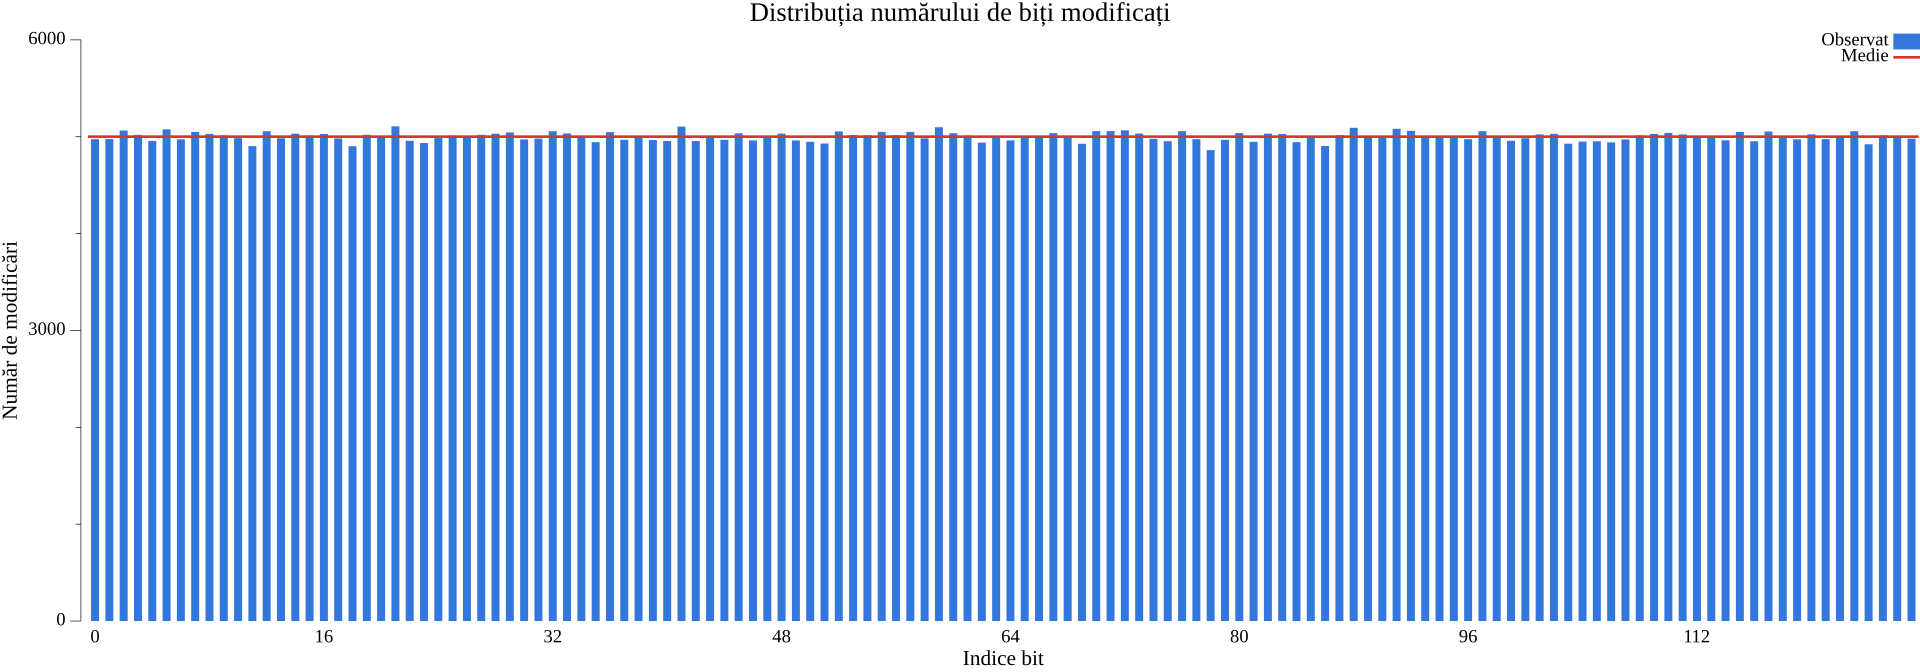
\includegraphics[width=\textwidth]{images/test-changed-bits-distribution.png}
    \caption{Frecvența modificării fiecărui bit al hash-ului pentru $N=10000$ mesaje}
    \label{fig:distributie-valori}
\end{figure}

Valoarea ideală pentru frecvența modificării fiecărui bit al hash-ului este de 50\% din numărul total de teste.
Astfel, pentru $N=10000$ mesaje, fiecare bit al hash-ului ar trebui să se schimbe de aproximativ 5000 de ori.
Conform graficului \ref{fig:distributie-valori}, se observă că frecvența modificării fiecărui bit al hash-ului se apropie foarte mult de această valoare ideală.
Valoarea minimă a frecvenței schimbării unui bit este de 4862, valoarea maximă este de 5107, iar media este de 5000.98.
Aceste rezultate indică faptul că valorile hash sunt distribuite uniform pe întreg spațiul de ieșire.

\subsection{Flexibilitate}
Având în vedere utilizarea construcției Sponge și a arborelui Merkle, funcția hash propusă admite o dimensiune a hash-ului final configurabilă.
Din punct de vedere teoretic, dimensiunea hash-ului poate fi de lungime arbitrară: 128 biți, 192 biți, 256 biți etc.
Numărul de runde intermediare variază în funcție de lungimea hash-ului final, deci pentru același mesaj, hash-urile de lungimi diferite vor fi complet diferite.

\subsection{Eficiența computațională}
Având în vedere că funcția hash propusă utilizează construcția Sponge și arborele Merkle, funcția poate fi ușor paralelizată.
De asemenea, utilizarea operațiilor pe biți, a operațiilor algebrice elementare și a tipurilor de date primitive sporește semnificativ viteza funcției.
Implementarea funcției hash propuse a fost realizată în două limbaje de programare diferite: Go și Rust.
Ambele implementări au fost optimizate pentru performanță, implementarea în Rust obținând viteze cu 30-40\% mai mari decât cea în Go.
Funcția hash propusă a fost testată pe seturi de date de dimensiuni variabile, cu un număr de nuclee alocate variabile.
Testele au fost efectuate pe trei sisteme diferite, cu configurații hardware diferite și cu sisteme de operare diferite:

\begin{itemize}
    \item Mac cu procesor Apple M2 Pro, 16GB RAM și macOS 15.6
    \item Laptop cu procesor AMD Ryzen 7 8845HS, 32GB RAM și Ubuntu 24.04
    \item Desktop cu procesor Intel Xeon Platinum 8370C, 64GB RAM și Windows 11
\end{itemize}
\section{Concluzii}
În această lucrare am proiectat și implementat o funcție hash bazată pe sisteme dinamice discrete haotice, construită în jurul structurii Sponge și al arborelui Merkle.
Analiza statistică prezentată în capitolul anterior confirmă faptul că funcția propusă posedă proprietăți criptografice solide.
Testele de confuzie și difuzie arată că o modificare minimă a mesajului de intrare determină o schimbare semnificativă a hash-ului.
Rezistența la coliziuni este, de asemenea, foarte bună: distribuția numărului de bytes egali și suma diferențelor absolute ale bytes-ilor se apropie de valorile teoretice, iar numărul de coliziuni observate este sub limita teoretică.
În plus, valorile hash sunt distribuite uniform pe întreg spațiul de ieșire, ceea ce împiedică atacurile bazate pe criptanaliză statistică.
Toate aceste rezultate sunt comparabile cu cele raportate de funcțiile hash consacrate din literatura de specialitate, ceea ce indică un nivel de securitate adecvat aplicațiilor criptografice moderne. \\

Pe lângă proprietățile criptografice, funcția hash propusă se remarcă prin viteza și eficiența sa pe sistemele cu mai multe nuclee.
Datorită arborelui Merkle, calculul hash-ului poate fi paralelizat eficient, viteza de procesare crescând aproape liniar cu numărul de nuclee alocate.
Pe sistemele moderne testate, funcția atinge viteze de procesare de ordinul sutelor de MB/s, comparabile cu cele ale funcțiilor hash utilizate la nivel de industrie, precum SHA-256 sau MD5.
Acest lucru este cu atât mai semnificativ cu cât funcțiile hash consacrate rulează pe un singur nucleu și beneficiază adesea de optimizări hardware dedicate. \\

Ca direcții viitoare de dezvoltare, o primă posibilitate ar fi implementarea funcției în limbajul C, în vederea obținerii unor viteze de procesare și mai mari.
O a doua direcție o constituie explorarea metodelor de optimizare hardware, prin care funcția ar putea fi accelerată suplimentar pe arhitecturi specializate.
În cele din urmă, o direcție promițătoare ar fi extinderea funcției hash într-o schemă completă de criptare și decriptare, valorificând proprietățile sistemelor dinamice haotice care stau la baza ei.

\printbibliography[heading=bibintoc]

\end{document}